\documentclass[10pt,aspectratio=169]{beamer}
\usepackage{realmadrid}

\usepackage{amsmath,amssymb}
\usepackage{booktabs}
\usepackage{array}
\usepackage{tikz}
\usetikzlibrary{positioning,arrows.meta,calc,shapes.geometric,fit,backgrounds}

% Tikz styles defined in preamble (not inside frames)
\tikzset{
  rmnode/.style={rectangle, draw=rmblue, thick, fill=rmpale,
                 minimum width=2.4cm, minimum height=0.9cm,
                 align=center, font=\small\bfseries, text=rmcharcoal},
  rmnodealt/.style={rectangle, draw=rmviolet, thick, fill=rmcream,
                    minimum width=2.4cm, minimum height=0.9cm,
                    align=center, font=\small\bfseries, text=rmcharcoal},
  rmnodegold/.style={rectangle, draw=rmgolddeep, thick, fill=rmgoldpale,
                     minimum width=2.4cm, minimum height=0.9cm,
                     align=center, font=\small\bfseries, text=rmcharcoal},
  rmarrow/.style={->, thick, rmblue, >=Stealth},
  rmarrowgold/.style={->, thick, rmgolddeep, >=Stealth},
}

\renewcommand{\rmfooter}{Codechella Madrid\,\textperiodcentered\,CUNEF\,\textperiodcentered\,May 2026}
\renewcommand{\rmsectionvenue}{CUNEF \textperiodcentered\ May 2026}

\title{The LaLonde Arc}
\author{Scott Cunningham}
\date{May 2026}

\begin{document}

% ====================================================================
% ACT I — THE HERETIC AND THE TRUTH
% ====================================================================

\rmtitleframe%
  {Sunset on the Bern\'abeu}%
  {The LaLonde Arc}%
  {How the field lost its faith, and how it found it again}%
  {Scott Cunningham}%
  {Codechella Madrid \textperiodcentered\ CUNEF \textperiodcentered\ May 2026}

% ---------- 2. Cold open ----------
\begin{frame}
  \frametitle{In 1986, a 32-year-old in Princeton asked the wrong question}
  \vspace{0.5cm}
  \begin{columns}[T,onlytextwidth]
    \begin{column}{0.55\textwidth}
      \rmquote{If economists swap the experimental controls for a
        non-experimental comparison group, do their methods still recover
        the true treatment effect?}{Robert LaLonde, \emph{AER}, 1986}
      \vspace{0.8em}

      \rmmeta{A practical question. A heretical implication. He answered: \rmkey{no}.}
    \end{column}
    \begin{column}{0.42\textwidth}
      \begin{block}{Why this mattered}
        Most causal claims in economics are observational. If matching the wrong way
        produces the wrong answer, then \rmblue{every observational claim is under suspicion}.
      \end{block}
    \end{column}
  \end{columns}
\end{frame}

% ---------- 3. The question that broke the field ----------
\begin{frame}
  \frametitle{The question that broke the field}
  \vspace{0.3cm}
  \begin{center}
    \resizebox{0.92\textwidth}{!}{%
    \begin{tikzpicture}[node distance=1.8cm]
      \node[rmnodegold] (truth)  {Experimental\\truth};
      \node[rmnode, right=of truth] (data)  {Same treated\\units};
      \node[rmnodealt, right=of data]  (swap) {Different\\controls (CPS)};
      \node[rmnode, right=of swap] (est)    {New\\estimate};
      \draw[rmarrow] (truth) -- (data);
      \draw[rmarrow] (data) -- (swap);
      \draw[rmarrow] (swap) -- (est);
    \end{tikzpicture}}
  \end{center}
  \vspace{0.3em}
  \begin{center}
    \rmblue{If the new estimate $=$ the truth, observational methods work.}\\[0.2em]
    \rmviolet{If not, the field has a problem.}
  \end{center}
\end{frame}

% ---------- 4. The experiment ----------
\begin{frame}
  \frametitle{The National Supported Work Demonstration (1975--1979)}
  \begin{columns}[T,onlytextwidth]
    \begin{column}{0.55\textwidth}
      \begin{itemize}
        \item Run by the \rmblue{Manpower Demonstration Research Corporation}
        \item Random assignment of long-term unemployed to subsidized jobs
        \item Treated: 9--12 months of guaranteed work + counseling
        \item \rmkey{Eligible applicants randomized}: 297 treated, 425 controls
        \item Outcome: 1978 annual earnings (\texttt{re78})
        \item Dehejia--Wahba (1999) restricted sample: \rmkey{185 treated, 260 controls}
      \end{itemize}
    \end{column}
    \begin{column}{0.42\textwidth}
      \begin{block}{Why it was credible}
        Not a textbook RCT. A real public program. Real frictions. \rmblue{Random
        assignment is the only thing rescuing the answer from selection bias.}
      \end{block}
    \end{column}
  \end{columns}
\end{frame}

% ---------- 5. The data: R chunk ----------
\begin{frame}[fragile]
  \frametitle{The data fits in 11 columns and 445 rows}
\begin{lstlisting}
library(haven); library(dplyr)
nsw <- read_dta("nsw_mixtape.dta")

#  data_id        treat   age  educ black hisp marr nodegree   re74   re75   re78
#  Dehejia-Wahba    1    37    11     1    0    1     1         0      0   9930
#  Dehejia-Wahba    1    22     9     0    1    0     1         0      0   3596
#  Dehejia-Wahba    1    30    12     1    0    0     0         0      0  24909

exp_att <- mean(nsw$re78[nsw$treat==1]) -
           mean(nsw$re78[nsw$treat==0])
#> $1,794
\end{lstlisting}
\vspace{-0.6em}
\rmmeta{One line of R. One number. The number we're going to compare everything else to.}
\end{frame}

% ---------- 6. The Stat: $1,794 ----------
\begin{frame}[plain]
  \rmstat{\$1{,}794}{The experimental ATT}
\end{frame}

% ---------- 7. Random assignment did its job ----------
\begin{frame}
  \frametitle{Random assignment did its job}
  \vspace{-0.4em}
  \begin{center}
    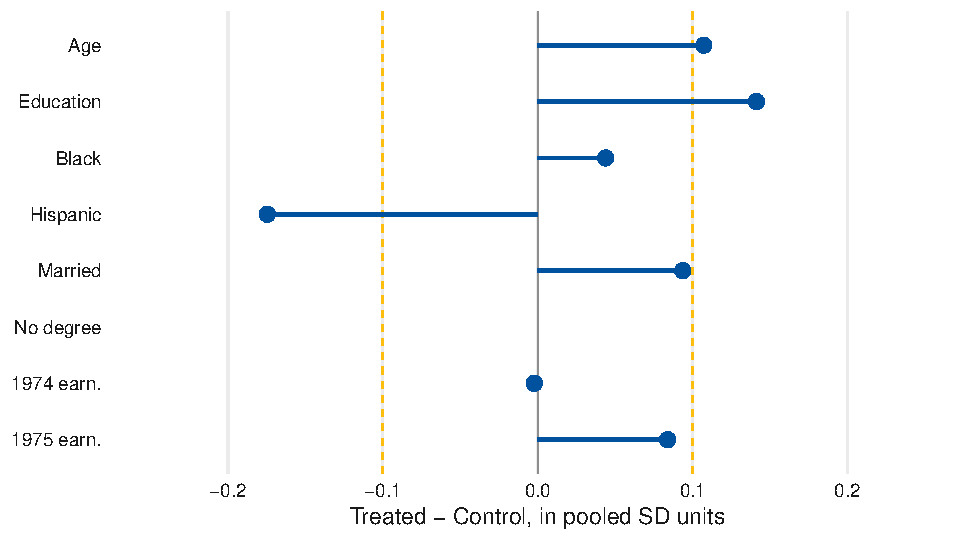
\includegraphics[width=0.74\textwidth]{figures/fig_balance.pdf}
  \end{center}
  \vspace{-0.6em}
  \rmmeta{Standardized differences in every covariate within $\pm 0.1$. The two
  groups are interchangeable on observables. We will leverage that fact, and then we will lose it.}
\end{frame}

% ---------- 8. Who was LaLonde ----------
\begin{frame}
  \frametitle{Who was Robert LaLonde?}
  \vspace{0.2cm}
  \begin{columns}[T,onlytextwidth]
    \begin{column}{0.55\textwidth}
      \begin{itemize}
        \item \rmblue{Princeton}, Ph.D.\ 1985 (advisor: Orley Ashenfelter)
        \item Assistant professor at Princeton, 1985--1991
        \item Later: Michigan State, then Chicago Harris (2000--2017)
        \item \rmkey{Died in 2018 at age 60} --- before he saw the full
        arc of what his \emph{AER} paper would set in motion
      \end{itemize}
      \vspace{0.5em}
      \rmmeta{He was a labor economist who became famous for testing
      labor econometrics. The provocation was his career's defining act.}
    \end{column}
    \begin{column}{0.42\textwidth}
      \begin{block}{The 1986 paper}
        \textit{Evaluating the Econometric Evaluations of Training Programs
        with Experimental Data}\\[0.3em]
        \rmblue{American Economic Review}, March 1986\\[0.3em]
        \rmgold{$\sim$11,000 citations} (as of 2025)
      \end{block}
    \end{column}
  \end{columns}
\end{frame}

% ====================================================================
% ACT II — THE CRISIS
% ====================================================================

\rmsection{The Swap}

% ---------- 9. The swap ----------
\begin{frame}
  \frametitle{The move: keep the treated, replace the controls}
  \vspace{0.2cm}
  \begin{center}
    \resizebox{0.94\textwidth}{!}{%
    \begin{tikzpicture}[node distance=1.4cm and 2.0cm]
      % Top row — the experimental control arm
      \node[rmnodegold] (exp)
        {NSW treated\\(185)};
      \node[rmnodegold, right=of exp] (ec)
        {NSW controls\\(260)};
      \node[rmnodegold, right=of ec] (eatt)
        {ATT: \$1{,}794};
      \draw[rmarrowgold] (exp) -- (ec);
      \draw[rmarrowgold] (ec) -- (eatt);

      % Bottom row — the swap
      \node[rmnode, below=of exp] (trt)
        {NSW treated\\(185)};
      \node[rmnodealt, right=of trt] (cps)
        {\textbf{CPS controls}\\(15{,}992)};
      \node[rmnode, right=of cps] (natt)
        {ATT: ?};
      \draw[rmarrow] (trt) -- (cps);
      \draw[rmarrow] (cps) -- (natt);

      \node[anchor=east, text=rmgold, font=\small\bfseries]
        at ([xshift=-0.4cm]exp.west) {EXPERIMENT};
      \node[anchor=east, text=rmviolet, font=\small\bfseries]
        at ([xshift=-0.4cm]trt.west) {SWAP};
    \end{tikzpicture}}
  \end{center}
  \vspace{0.1em}
  \begin{center}
    \rmmeta{Same treated units. Different counterfactual. Standard econometric methods.}
  \end{center}
\end{frame}

% ---------- 10. Horserace ----------
\begin{frame}
  \frametitle{The naïve methods collapse}
  \vspace{-0.8em}
  \begin{center}
    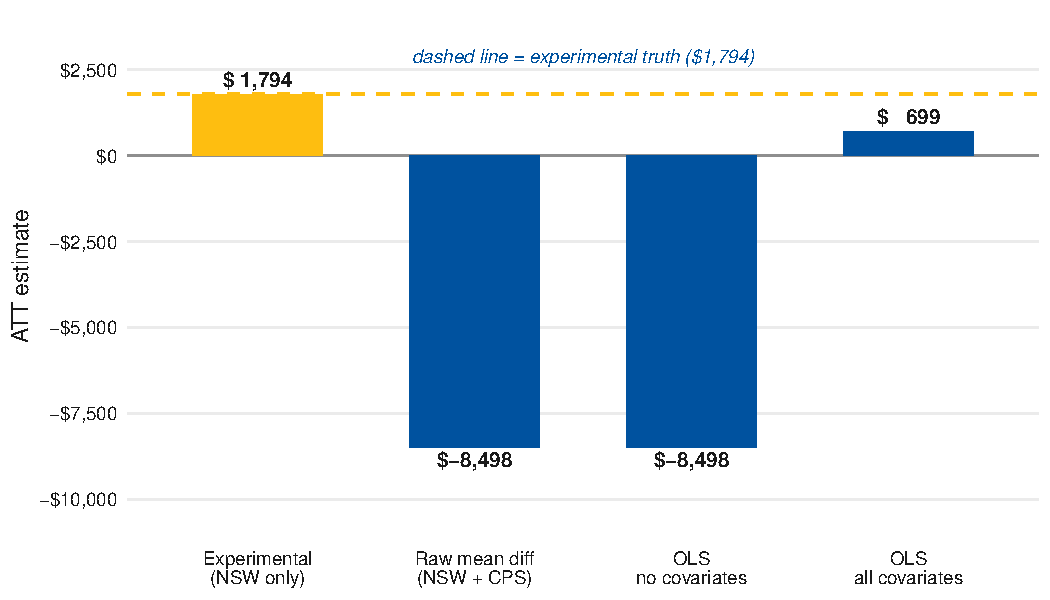
\includegraphics[width=0.80\textwidth]{figures/fig_lalonde_horserace.pdf}
  \end{center}
  \vspace{-0.8em}
  \rmmeta{Every standard estimator misses by thousands of dollars. OLS-with-controls comes closest --- and is still off by \$1{,}095.}
\end{frame}

% ---------- 11. STAT: bias ----------
\begin{frame}[plain]
  \rmstat{$-\$8{,}498$}{Raw bias from the CPS swap}
\end{frame}

% ---------- 12. The skeptic's reading ----------
\begin{frame}
  \frametitle{The skeptic's reading was the obvious one}
  \vspace{0.2cm}
  \rmquote{If a state-of-the-art econometric toolkit, given a clean RCT to
  shadow, cannot recover the experimental answer --- what business do we
  have using these methods on observational data alone?}{the field, 1986}
  \vspace{0.2em}
  \begin{block}{What \rmkey{cannot} be fixed}
    Functional form. Controls. Significance stars. Bigger samples.
  \end{block}
  \begin{block}{What \rmkey{must} be re-thought}
    Identification. Selection. The assumption behind OLS.
  \end{block}
\end{frame}

% ---------- 13. The long silence ----------
\begin{frame}
  \frametitle{Then nothing happened for thirteen years}
  \vspace{0.4cm}
  \begin{center}
    \begin{tikzpicture}[x=1.0cm, y=1.0cm]
      % Timeline
      \draw[rmblue, line width=1.2pt] (0,0) -- (12,0);
      % Tick marks
      \foreach \x/\year in {0/1986, 4/1990, 8/1995, 11/1999, 12/2001} {
        \draw[rmblue, line width=0.8pt] (\x, -0.15) -- (\x, 0.15);
        \node[below=2pt, text=rmcharcoal, font=\footnotesize] at (\x, -0.15) {\year};
      }
      % Pulses
      \node[anchor=south, text=rmviolet, font=\footnotesize\itshape] at (0, 0.2)
        {LaLonde};
      \node[anchor=south, text=rmblue, font=\footnotesize\itshape] at (11, 0.2)
        {Dehejia--Wahba};
      \node[anchor=south, text=rmblue, font=\footnotesize\itshape] at (8.2, 1.0)
        {Heckman--Ichimura--Todd};
      \draw[rmblue, dashed, line width=0.4pt] (8.2, 0.9) -- (8.2, 0.18);
      % Annotation of the silence
      \node[anchor=center, text=rmash, font=\footnotesize\itshape]
        at (5.5, -0.9) {\textit{(thirteen years)}};
      \draw[rmash, line width=0.3pt] (0.4, -0.55) -- (10.6, -0.55);
    \end{tikzpicture}
  \end{center}
  \vspace{0.8em}
  \rmmeta{The toolkit existed: Heckman (1979), Rosenbaum--Rubin (1983), matching. \rmblue{Off the shelf, none of it closed the gap.}}
\end{frame}

% ---------- 14. What the field had but couldn't use ----------
\begin{frame}
  \frametitle{The 1986 toolkit could adjust --- but it could not diagnose}
  \vspace{0.6cm}
  \begin{center}
    \rmblue{Heckman (1979)}\quad\textperiodcentered\quad
    \rmblue{Rosenbaum--Rubin (1983)}\quad\textperiodcentered\quad
    \rmblue{standard matching}
  \end{center}
  \vspace{1.0em}
  \begin{block}{The gap}
    Every method on the shelf in 1986 \textit{adjusted} for observed $X$. None of them told you
    \rmkey{whether the adjustment had worked}. That is what LaLonde demanded --- and what the
    field couldn't deliver for the next decade.
  \end{block}
\end{frame}

% ---------- 15. The first crack ----------
\begin{frame}
  \frametitle{The first crack: Dehejia \& Wahba (1999, JASA)}
  \vspace{0.3cm}
  \begin{columns}[T,onlytextwidth]
    \begin{column}{0.55\textwidth}
      \begin{itemize}
        \item Re-ran LaLonde, but with \rmblue{propensity score matching}
        \item Subsampled NSW to the 185-treated/260-control overlap window
        \item PSM brought the ATT \rmkey{back to roughly \$1{,}600--\$1{,}900}
        \item First published demonstration that an observational method could
        recover the experimental answer
      \end{itemize}
    \end{column}
    \begin{column}{0.42\textwidth}
      \begin{block}{But matching alone is fragile}
        \begin{itemize}\setlength{\itemsep}{0pt}
          \item Sensitive to the PS specification
          \item Sensitive to which units are in the support window
          \item Smith \& Todd (2005): change covariates, change the answer
        \end{itemize}
      \end{block}
    \end{column}
  \end{columns}
\end{frame}

% ---------- 16. The overlap figure ----------
\begin{frame}
  \frametitle{The treated and controls live in different worlds}
  \vspace{-0.6em}
  \begin{center}
    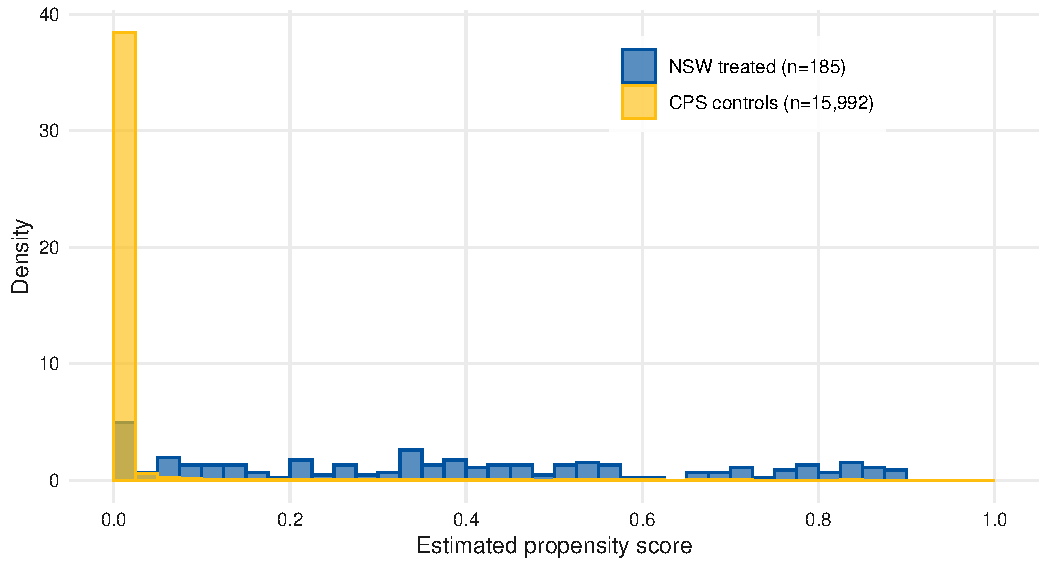
\includegraphics[width=0.78\textwidth]{figures/fig_pscore_overlap.pdf}
  \end{center}
  \vspace{-0.6em}
  \rmmeta{93\% of CPS controls have $\hat{p}<0.01$. \rmblue{This is the geometry
  that breaks matching} --- and the geometry the next two methods will navigate.}
\end{frame}

% ====================================================================
% ACT III — TWO ROADS HOME
% ====================================================================

\rmsection{Heckman--Ichimura--Todd (1997)}

% ---------- 17. Who they were ----------
\begin{frame}
  \frametitle{Who were Heckman, Ichimura, and Todd?}
  \vspace{0.2em}
  \begin{columns}[T,onlytextwidth]
    \begin{column}{0.32\textwidth}
      \begin{block}{Heckman}
        Chicago, the Nobel laureate (2000)\\
        \rmmeta{Selection theory, training-program evaluation, the field's senior figure}
      \end{block}
    \end{column}
    \begin{column}{0.32\textwidth}
      \begin{block}{Ichimura}
        Pittsburgh, then Tokyo\\
        \rmmeta{Semiparametric estimation, single-index models}
      \end{block}
    \end{column}
    \begin{column}{0.32\textwidth}
      \begin{block}{Todd}
        Penn, then Chicago Booth\\
        \rmmeta{Heckman student. The empirical engine of the trio.}
      \end{block}
    \end{column}
  \end{columns}
  \vspace{0.5em}
  \rmmeta{\rmblue{\textit{Review of Economic Studies}, October 1997}: a 50-page paper that
  reframed matching as a diagnostic problem, not just an estimator.}
\end{frame}

% ---------- 18. The diagnostic ----------
\begin{frame}
  \frametitle{The HIT diagnostic: total bias has three sources}
  \vspace{0.2cm}
  \begin{center}
    \resizebox{0.86\textwidth}{!}{%
    \begin{tikzpicture}[node distance=1.0cm and 1.2cm]
      \node[rmnodegold] (B) {$B = E[Y^0\,|\,D{=}1] - E[Y^0\,|\,D{=}0]$};
      \node[rmnode, below left=of B, xshift=-1.0cm]  (B1) {$B_1$: non-overlap};
      \node[rmnode, below=of B]                       (B2) {$B_2$: density};
      \node[rmnode, below right=of B, xshift=1.0cm]  (B3) {$B_3$: selection};
      \draw[rmarrow] (B) -- (B1);
      \draw[rmarrow] (B) -- (B2);
      \draw[rmarrow] (B) -- (B3);
      \node[below=0.35cm of B1, text=rmash, font=\scriptsize, text width=3cm, align=center]
        {Treated outside control support};
      \node[below=0.35cm of B2, text=rmash, font=\scriptsize, text width=3cm, align=center]
        {Different distribution of $X$};
      \node[below=0.35cm of B3, text=rmash, font=\scriptsize, text width=3cm, align=center]
        {Selection on \textbf{unobservables}};
    \end{tikzpicture}}
  \end{center}
  \vspace{0.4em}
  \begin{center}
    \rmblue{Matching can fix $B_1$ and $B_2$.}\quad
    \rmviolet{Only conditional DiD can fix $B_3$.}
  \end{center}
\end{frame}

% ---------- 19. The key insight: A-5 is weaker ----------
\begin{frame}
  \frametitle{The key insight: conditional parallel trends is weaker}
  \vspace{0.4cm}
  \begin{itemize}
    \item \rmblue{Matching} requires $E[Y^0\,|\,X, D{=}1] = E[Y^0\,|\,X, D{=}0]$ \\
      \rmmeta{\textbf{Levels} of the untreated outcome match conditional on $X$.}
    \item \rmblue{Conditional DiD} requires only \\
      \rmkey{$E[Y^0_t - Y^0_{t'}\,|\,X, D{=}1] = E[Y^0_t - Y^0_{t'}\,|\,X, D{=}0]$}\\
      \rmmeta{\textbf{Changes} match conditional on $X$. Level differences are allowed.}
  \end{itemize}
  \vspace{0.5em}
  \begin{block}{What HIT showed empirically}
    On the JTPA data with multiple comparison groups: matching's assumption (\textbf{A-3}, \textbf{A-4})
    was \rmblue{rejected at $p<0.001$}. The DiD assumption (\textbf{A-5}) was \rmkey{not rejected}.
  \end{block}
\end{frame}

% ---------- 20. The estimator: local linear + DiD ----------
\begin{frame}
  \frametitle{The estimator: local-linear kernel matching on $\Delta Y$}
  \vspace{0.3cm}
  \begin{enumerate}
    \item Fit $\hat p(X) = \Pr(D{=}1\,|\,X)$ via logit
    \item Restrict to common support: $\hat p \in [\hat p_{\min}, \hat p_{\max}]$
    \item For each treated $i$: estimate $\widehat{E}[\Delta Y\,|\,\hat p, D{=}0]$
          using \rmblue{Fan's (1992) local linear regression}
    \item Average $\Delta Y_i - \widehat{E}[\Delta Y_i\,|\,\hat p_i, D{=}0]$
          over treated units
  \end{enumerate}
  \vspace{0.5em}
  \begin{block}{Why each step matters}
    \begin{itemize}\setlength{\itemsep}{0pt}
      \item Step 2 fixes $B_1$ (non-overlap)
      \item Step 3 fixes $B_2$ (density weighting) via kernel re-weighting
      \item Step 4 fixes $B_3$ if A-5 holds (conditional parallel trends)
    \end{itemize}
  \end{block}
\end{frame}

% ---------- 21. R CODE ----------
\begin{frame}[fragile]
  \frametitle{Twelve lines of R get you to \$2{,}051}
\begin{lstlisting}
ps_mod <- glm(treat ~ age + I(age^2) + educ + black + hisp +
              marr + nodegree + re74 + re75 + I(re74^2) + I(re75^2),
              data=cps, family=binomial)
cps$ps <- predict(ps_mod, type="response")
cs <- subset(cps, ps>=min(ps[treat==1]) & ps<=max(ps[treat==1]))
trt  <- subset(cs, treat==1);  trt$dy  <- trt$re78  - trt$re75
ctrl <- subset(cs, treat==0);  ctrl$dy <- ctrl$re78 - ctrl$re75
h <- 0.9 * min(sd(ctrl$ps), IQR(ctrl$ps)/1.34) * length(ctrl$ps)^(-1/5)
trt$dy0 <- sapply(trt$ps, local_linear, x=ctrl$ps, y=ctrl$dy, h=h)
hit_att <- mean(trt$dy - trt$dy0)
#> $2,051
\end{lstlisting}
\end{frame}

% ---------- 22. The HIT road plot ----------
\begin{frame}
  \frametitle{The first road home}
  \vspace{-0.2em}
  \begin{center}
    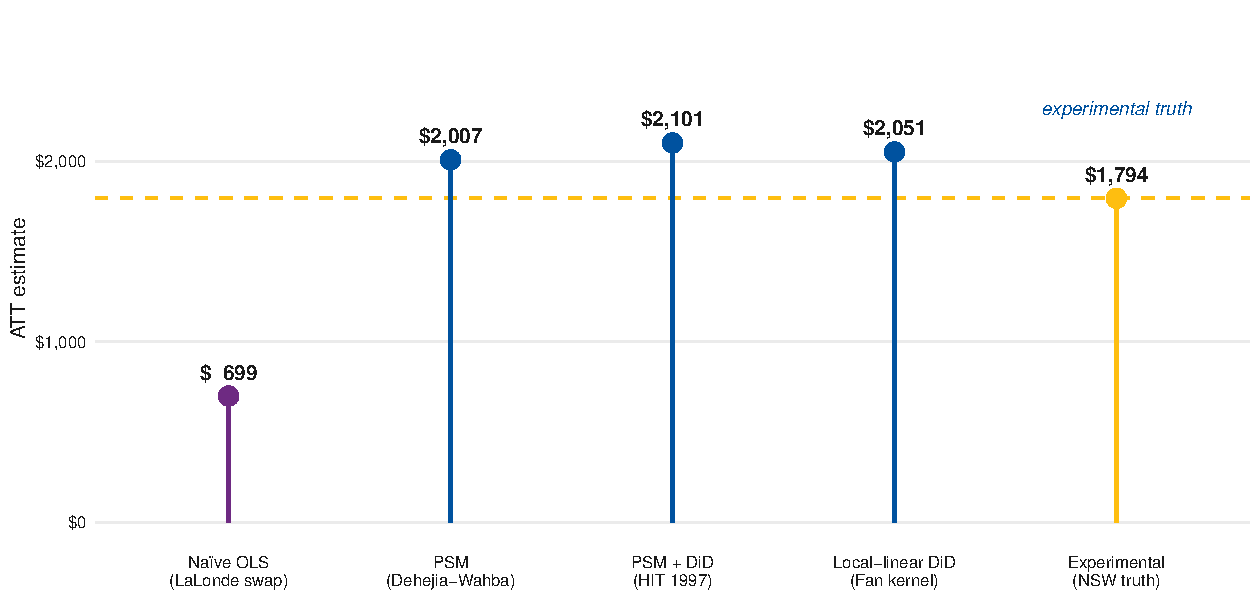
\includegraphics[width=0.88\textwidth]{figures/fig_hit_road.pdf}
  \end{center}
\end{frame}

% ---------- 23. STAT: $2,051 ----------
\begin{frame}[plain]
  \rmstat{\$2{,}051}{HIT recovers the experimental neighborhood}
\end{frame}

\rmsection{Abadie (2005)}

% ---------- 24. Who Abadie was ----------
\begin{frame}
  \frametitle{Who is Alberto Abadie?}
  \vspace{0.3cm}
  \begin{columns}[T,onlytextwidth]
    \begin{column}{0.55\textwidth}
      \begin{itemize}
        \item MIT Ph.D.\ 1999 (advisor: Joshua Angrist)
        \item Harvard Kennedy School 2000--2018, then MIT economics
        \item \rmkey{Inventor of the synthetic control method} (with Gardeazabal, 2003)
        \item Co-developer of the design-based standard-error literature
        (Abadie--Athey--Imbens--Wooldridge, 2020)
      \end{itemize}
      \vspace{0.5em}
      \rmmeta{A Spaniard. From the Basque country.
      Codechella Madrid would not exist without him.}
    \end{column}
    \begin{column}{0.42\textwidth}
      \begin{block}{The 2005 paper}
        \textit{Semiparametric Difference-in-Differences Estimators}\\[0.3em]
        \rmblue{Review of Economic Studies}, January 2005\\[0.3em]
        \rmgold{$\sim$3{,}500 citations}
      \end{block}
    \end{column}
  \end{columns}
\end{frame}

% ---------- 25. The elegance: re-weight instead of match ----------
\begin{frame}
  \frametitle{Re-weight instead of match}
  \vspace{0.3cm}
  \begin{itemize}
    \item HIT estimates \rmblue{one function for the treated} and \rmblue{one for the controls},
      then differences them
    \item Abadie estimates \rmkey{one function only} --- the propensity score $p(X)$ ---
      and uses it as a \rmblue{re-weighting kernel}
  \end{itemize}
  \vspace{0.5em}
  \begin{block}{The headline identity}
    \[
      \mathrm{ATT}\ =\ \frac{1}{\Pr(D{=}1)}\
      E\!\left[\,\frac{D - p(X)}{1 - p(X)}\cdot \big(Y_{1} - Y_{0}\big)\right]
    \]
    \rmmeta{One propensity score. One weighted mean of temporal differences. Done.}
  \end{block}
\end{frame}

% ---------- 26. R CODE for Abadie ----------
\begin{frame}[fragile]
  \frametitle{Five lines of R get you to \$1{,}642}
\begin{lstlisting}
ps_mod <- glm(treat ~ age + I(age^2) + educ + black + hisp +
              marr + nodegree + re74 + re75 + I(re74^2) + I(re75^2),
              data=cps, family=binomial)
cps$ps <- predict(ps_mod, type="response")
cs <- subset(cps, ps>0.01 & ps<0.99)
cs$dY <- cs$re78 - cs$re75
abadie_att <- mean( ((cs$treat - cs$ps)/(1 - cs$ps)) * cs$dY ) / mean(cs$treat)
#> $1,642
\end{lstlisting}
\end{frame}

% ---------- 27. The Abadie road plot ----------
\begin{frame}
  \frametitle{The second road home}
  \vspace{-0.2em}
  \begin{center}
    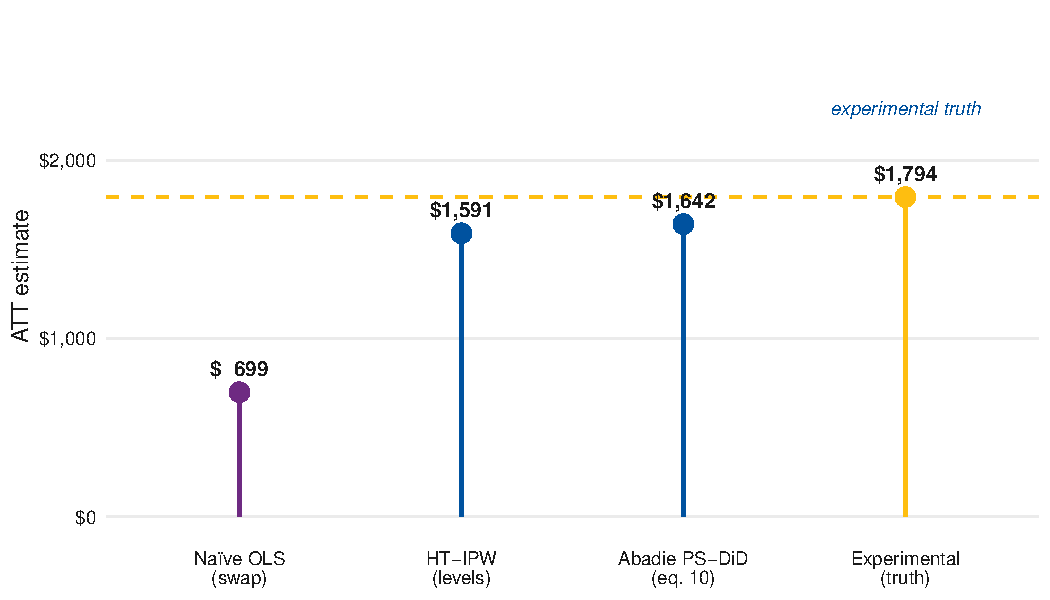
\includegraphics[width=0.88\textwidth]{figures/fig_abadie_road.pdf}
  \end{center}
\end{frame}

% ---------- 28. STAT: $1,642 ----------
\begin{frame}[plain]
  \rmstat{\$1{,}642}{Abadie also recovers the experimental neighborhood}
\end{frame}

% ---------- 29. The synthesis ----------
\begin{frame}
  \frametitle{Two different machines, same destination}
  \vspace{0.4cm}
  \begin{tabular}{lrr}
\toprule
\textbf{Method} & \textbf{ATT} & \textbf{Gap vs.\ truth} \\
\midrule
\textit{LaLonde's swap (the crisis)} & & \\
\quad OLS, all covariates              & \$699 & \textcolor{rmburgundy}{\$-1,095} \\
\midrule
\textit{The two roads home (the resolution)} & & \\
\quad Heckman--Ichimura--Todd (1997)    & \$2,051 & \$257 \\
\quad Abadie (2005) PS-weighted DiD     & \$1,642 & \$-152 \\
\midrule
\textit{Experimental benchmark}        & \textcolor{rmgold}{\textbf{\$1,794}} & --- \\
\bottomrule
\end{tabular}

  \vspace{0.8em}
  \begin{center}
    \rmblue{Match-then-difference} and \rmblue{re-weight-and-difference} converge
    on the same neighborhood as the experimental answer.\\[0.2em]
    \rmmeta{When two independent roads built a decade apart arrive at the
    same place, the answer is in.}
  \end{center}
\end{frame}

% ---------- 29b. Devil's Advocate slide (rhetoric audit critical fix) ----------
\begin{frame}
  \frametitle{The roads converge on a neighborhood, not a point}
  \vspace{0.4cm}
  \begin{itemize}
    \item HIT delivers \rmkey{\$2{,}051}; Abadie delivers \rmkey{\$1{,}642}.
    The two roads disagree with each other by \rmblue{\$409}.
    \item That gap is the price of specification choice: the propensity-score functional form,
    the trimming rule, the kernel bandwidth.
    \item \rmblue{Smith \& Todd (2005, JoE)}: change the covariates, change the answer.
    Neither method is a free lunch.
  \end{itemize}
  \vspace{0.4em}
  \begin{block}{What is actually robust}
    Not the third significant digit. What is robust is the \rmkey{direction}
    (\$1{,}500--\$2{,}100, not negative) and the \rmkey{order of magnitude} (thousands,
    not tens of thousands). That is enough to declare LaLonde's challenge answered.
  \end{block}
\end{frame}

% ====================================================================
% ACT IV — WHY THESE DATES? WHY THESE PEOPLE?
% ====================================================================

\rmsection{Why Then?}

% ---------- 30. Why 1997, not 1987 or 1995 ----------
\begin{frame}
  \frametitle{Why HIT in 1997 --- not 1987, not 1995?}
  \vspace{0.3cm}
  \begin{itemize}
    \item \rmblue{Rosenbaum--Rubin (1983)} gave the field the propensity score.
      \rmmeta{But it took a decade to be absorbed.}
    \item \rmblue{Fan (1992, 1993)} made local-linear kernel regression respectable.
      \rmmeta{HIT needed this --- ordinary kernel matching has bias that LL eliminates.}
    \item \rmblue{Card--Krueger (1994)} revived DiD as a serious identification tool.
      \rmmeta{Suddenly, the idea of differencing across time was in the air again.}
    \item \rmblue{Eleven years} since LaLonde had passed. The unsolved challenge
      had become a \rmkey{career-defining target} for an ambitious empirical team.
  \end{itemize}
\end{frame}

% ---------- 31. The Heckman lab ----------
\begin{frame}
  \frametitle{The Heckman lab in the 1990s}
  \vspace{0.3cm}
  \begin{itemize}
    \item Heckman won the Nobel in 2000 for selection models, but his Chicago lab
      in the 1990s was a \rmblue{dissertation factory}
    \item Dissertations that came out of it: Petra Todd, Hidehiko Ichimura, Jeffrey Smith
    \item The lab had been chewing on the LaLonde puzzle for years
    \item The 1997 paper was followed by \rmblue{Heckman--Ichimura--Smith--Todd (1998, ReStud)}
      --- the companion piece with the full theory
  \end{itemize}
  \vspace{0.5em}
  \begin{block}{The lesson}
    Big methodological breakthroughs come from \rmkey{labs}, not lone genius.
    Heckman gave the architecture; Ichimura and Todd built it.
  \end{block}
\end{frame}

% ---------- 32. Why 2005 ----------
\begin{frame}
  \frametitle{Why Abadie in 2005 --- not 1995, not 2015?}
  \vspace{0.3cm}
  \begin{itemize}
    \item \rmblue{Hirano--Imbens--Ridder (2003)} showed PS weighting is semiparametrically
      efficient. \rmmeta{Suddenly re-weighting had a respectability that matching alone lacked.}
    \item \rmblue{Bertrand--Duflo--Mullainathan (2004)} broke DiD inference and
      forced the field to rebuild the standard error machine.
      \rmmeta{Abadie's PS-DiD slotted into the rebuild.}
    \item \rmblue{Abadie--Gardeazabal (2003)} --- synthetic control. Abadie himself
      had spent two years thinking about \rmkey{weights as the solution to identification},
      not matches.
    \item The 2005 paper was the natural synthesis: take HIT's conditional DiD
      assumption, replace the matching step with re-weighting, prove the asymptotics.
  \end{itemize}
\end{frame}

% ---------- 33. Notation: A-4 vs A-5 (compressed per rhetoric audit) ----------
\begin{frame}
  \frametitle{A-5 is strictly weaker than A-4 --- and that is the whole story}
  \vspace{0.6cm}
  \begin{center}
    \begin{tikzpicture}[node distance=0.8cm and 1.8cm]
      \node[rmnode, text width=4.4cm, minimum height=1.5cm] (A4)
        {\textbf{A-4} \ (matching)\\[0.2em]
         $E[Y^0\,|\,X, D{=}1] = E[Y^0\,|\,X, D{=}0]$\\[0.2em]
         {\scriptsize\itshape \rmgold{levels} match}};
      \node[rmnodegold, text width=4.6cm, minimum height=1.5cm, right=of A4] (A5)
        {\textbf{A-5} \ (conditional DiD)\\[0.2em]
         $E[\Delta Y^0\,|\,X, D{=}1] = E[\Delta Y^0\,|\,X, D{=}0]$\\[0.2em]
         {\scriptsize\itshape \rmgold{changes} match; level shifts allowed}};
      \draw[rmarrowgold, line width=1.1pt] (A4) -- node[above, text=rmcharcoal, font=\small\itshape] {implies} (A5);
    \end{tikzpicture}
  \end{center}
  \vspace{0.8em}
  \rmmeta{Selection on time-invariant unobservables is allowed under \textbf{A-5}. The
  level of $Y^0$ can differ between treated and controls --- only the time path must match.
  That weakening is what HIT proved you needed, and what Abadie 2005 then leveraged.}
\end{frame}

% ---------- 34. The Abadie weight ρ₀ ----------
\begin{frame}
  \frametitle{The Abadie weight $\rho_0$}
  \vspace{0.2cm}
  Define $\rho_0 = (D - p(X)) / (p(X)\,(1 - p(X)))$. Then under \textbf{A-2} and \textbf{A-5},
  \[
    E\!\left[\rho_0\cdot(Y_1 - Y_0)\,\big|\,X\right]\ =\ E[Y^1 - Y^0 \mid X, D{=}1]
  \]
  \begin{block}{Reading the weight}
    \begin{itemize}\setlength{\itemsep}{0pt}
      \item Treated ($D=1$): $\rho_0 = 1/p(X)$ --- upweight rare-treated cells
      \item Controls ($D=0$): $\rho_0 = -1/(1-p(X))$ --- downweight common controls
      \item $E[\rho_0\mid X] = 0$ --- weights sum to zero in expectation
    \end{itemize}
  \end{block}
  \begin{center}\rmmeta{And so --- back to the three numbers.}\end{center}
\end{frame}

% ====================================================================
% CLOSING
% ====================================================================

% ---------- 35. Final stat slide: three numbers ----------
\begin{frame}[plain]
  \begin{tikzpicture}[remember picture, overlay]
    \node[anchor=center, text=rmblue, font=\bfseries\fontsize{16pt}{18pt}\selectfont]
      at ([yshift=2.6cm]current page.center) {Three numbers, one truth};
    \node[anchor=east, text=rmgold, font=\bfseries\fontsize{52pt}{58pt}\selectfont]
      at ([xshift=-1.0cm,yshift=0.6cm]current page.center) {\$1{,}794};
    \node[anchor=center, text=rmash, font=\fontsize{10pt}{12pt}\selectfont\itshape]
      at ([yshift=-0.55cm]current page.center) {is roughly equal to};
    \node[anchor=west, text=rmblue, font=\bfseries\fontsize{36pt}{40pt}\selectfont]
      at ([xshift=1.0cm,yshift=0.6cm]current page.center) {\$2{,}051};
    \node[anchor=west, text=rmblue, font=\bfseries\fontsize{36pt}{40pt}\selectfont]
      at ([xshift=1.0cm,yshift=-1.4cm]current page.center) {\$1{,}642};
    \node[anchor=center, text=rmash, font=\fontsize{9pt}{11pt}\selectfont]
      at ([yshift=-2.6cm]current page.center)
      {Experimental \ $\approx$ \ Heckman--Ichimura--Todd (1997) \ $\approx$ \ Abadie (2005)};
    \draw[rmgold, line width=0.8pt]
      ([xshift=-3.5cm, yshift=-2.0cm]current page.center)
      -- ([xshift=3.5cm, yshift=-2.0cm]current page.center);
  \end{tikzpicture}
\end{frame}

% ---------- 36. Closing line ----------
\begin{frame}[plain]
  \begin{tikzpicture}[remember picture, overlay]
    \fill[rmblue] (current page.south west) rectangle (current page.north east);
    \node[anchor=center, text=rmgold, font=\bfseries\fontsize{10pt}{12pt}\selectfont]
      at ([yshift=2.0cm]current page.center) {\MakeUppercase{the lalonde arc}};
    \node[anchor=center, text=rmwhite, text width=0.78\paperwidth, align=center,
          font=\itshape\fontsize{22pt}{28pt}\selectfont]
      at ([yshift=0.2cm]current page.center)
      {When two roads built a decade apart\\arrive at the same \$1{,}794,\\the field has its answer.};
    \draw[rmgold, line width=0.8pt]
      ([xshift=-2.5cm, yshift=-2.0cm]current page.center)
      -- ([xshift=2.5cm, yshift=-2.0cm]current page.center);
    \node[anchor=south, text=rmgold, font=\fontsize{8pt}{10pt}\selectfont\itshape]
      at ([yshift=0.8cm]current page.south) {Codechella Madrid 2026 \textperiodcentered\ CUNEF};
  \end{tikzpicture}
\end{frame}

\end{document}
